\section{Tematyka pracy}
%------------------------------------------------

\begin{frame}
\frametitle{Symulacja robotów}
\begin{block}{Cel symulacji}
	Głównym celem symulacji robotów jest zapewnienie bezpieczeństwa:
	\begin{itemize}
		\item ludziom
		\item środowisku
		\item systemowi robotycznemu
	\end{itemize}
\end{block}
\end{frame}

%------------------------------------------------

\begin{frame}
	\frametitle{Niebezpieczeństwa}
	Brak przetestowania systemu przed uruchomieniem w rzeczywistości może powodować \cite{bezpieczenstwo}:
	\begin{itemize}
		\item wydatki nieuwzględnione w początkowym kosztorysie
		\item opóźnienia w eksperymentach
		\item uszkodzenie sprzętu
		\item obrażenia u ludzi
	\end{itemize}
\end{frame}

%------------------------------------------------

\begin{frame}
\frametitle{Porównanie symulacji z działaniem w rzeczywistości}
\begin{figure}
	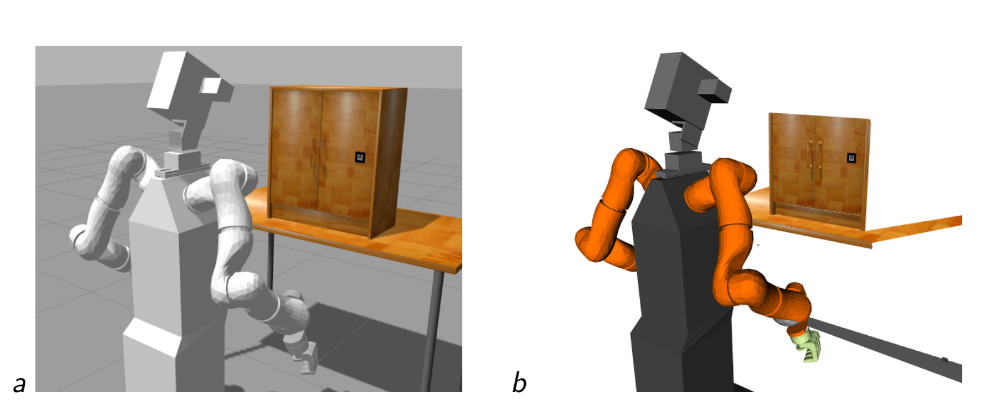
\includegraphics[scale=0.35]{./images/otwieranie_gz.png}
	\setcaptioncitation{T.Winiarski. Wybrane aspekty bezpieczeństwa w badaniach robotów usługowych \cite{bezpieczenstwo}}
	\caption{Zadanie otwierania drzwi w a) symulatorze Gazebo b) w narzędziu Rviz}
	\end{figure}
\end{frame}

%------------------------------------------------

\begin{frame}
\frametitle{Porównanie symulacji z działaniem w rzeczywistości}
\begin{figure}
	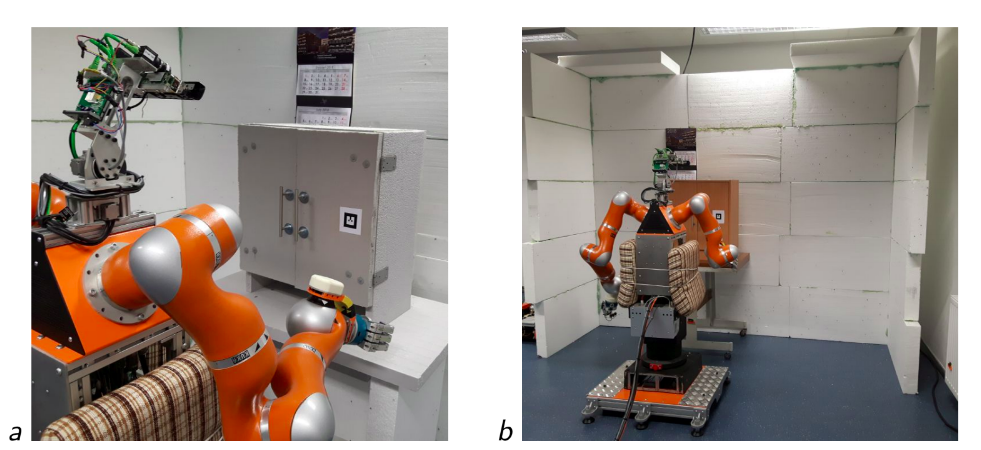
\includegraphics[scale=0.35]{./images/otwieranie_real.png}
	\setcaptioncitation{T.Winiarski. Wybrane aspekty bezpieczeństwa w badaniach robotów usługowych \cite{bezpieczenstwo}}
	\caption{Zadanie otwierania drzwi w a) środowisku podatnym b) w środowisku rzeczywistym}
	\end{figure}
\end{frame}

%------------------------------------------------

\begin{frame}
	\frametitle{Symulator Gazebo}
	Symulator Gazebo umożliwia:
	\begin{itemize}
		\item symulację robotów w otwartych i zamkniętych środowiskach
		\item tworzenie własnych wtyczek dla własnych efektorów i czujników 
		\item integrację z Robot Operating System
		\item tworzenie własnych modeli obiektów w popularnych formatach SDF i URDF
		\item symulowanie światów przy użyciu różnych silników fizyki 
	\end{itemize}
	\bigskip \medskip
	\begin{figure}
		
\includegraphics[scale=0.3]{./images/gazebo.png}
		\setcaptioncitation{\texttt{gazebosim.org}}
		\caption{Logo symulatora Gazebo}
	\end{figure}
\end{frame}

%------------------------------------------------

\begin{frame}
	\frametitle{Robot Operating System}
	\begin{block}{ROS}
		\textit{Robot Operating System} jest otwartoźródłowym środowiskiem programistycznym do programowania robotów.
		Umożliwia rozproszoną komunikację pomiędzy procesami oraz reużywalność kodu.
	\end{block}
	\medskip
	\begin{figure}
		
\includegraphics[scale=0.2]{./images/ros-melodic.png}
		\setcaptioncitation{\texttt{ros.org}}
		\caption{Logo systemu ROS Melodic Morenia}
	\end{figure}
\end{frame}

%------------------------------------------------

\begin{frame}
	\frametitle{Robot Operating System}
	\begin{figure}
		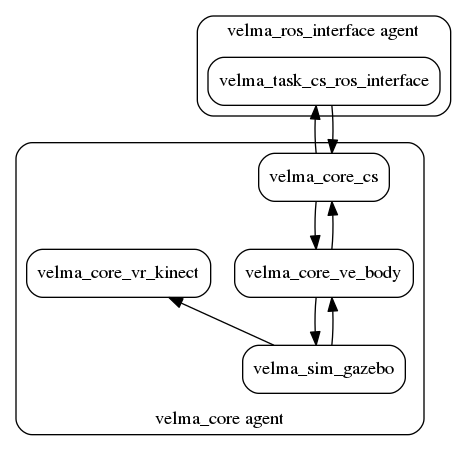
\includegraphics[scale=0.4]{./images/system-sim.png}
		\setcaptioncitation{\texttt{rcprg-ros-pkg.github.io/velma\_docs/}  \cite{docsVelma}}
		\caption{Podstawowa struktura sterownika robota Velma w symulacji}
	\end{figure}
\end{frame}

%------------------------------------------------

\begin{frame}
	\frametitle{Robot Operating System}
	\begin{figure}
		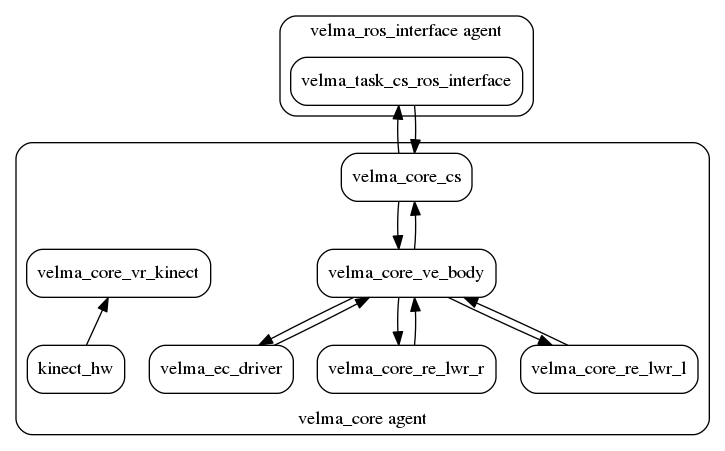
\includegraphics[scale=0.4]{./images/system-hw.png}
		\setcaptioncitation{\texttt{rcprg-ros-pkg.github.io/velma\_docs/}  \cite{docsVelma}}
		\caption{Podstawowa struktura sterownika rzeczywistego robota Velma}
	\end{figure}
\end{frame}
	
%------------------------------------------------
